Откачаем воздух из полости спектрометра, включим вакуумметр, ПЭВМ, формирователь
импульсов и питание магнитной линзы. Уменьшим ток через магнитную линзу до нуля.

Проведем измерение $\beta$-спектра, изменяя ток в магнитной линзе, при каждом
значении тока будем измерять число попаданий частиц в детектор за $100$ секунд.
Значения сразу будут приведены в виде $N = \frac{N'}{t}$ -- число частиц в
единицу времени.

Измерим фон:

\begin{table}[h!]
  \caption{Измерения фона}
  \begin{center}
    \begin{tabular}{| c | c | c |}
      \hline
      $I$, А & $0$ & $4.2$\\
      \hline
      $N_{\text{Ф}}$, 1/c & 1.32 & 0.71\\
      \hline
    \end{tabular}
  \end{center}
\end{table}

Измерим сам спектр и проведем вычет фона из числа частиц. Отложим на графике
экспериментальные точки в осях $I$, $N - N_{\text{Ф}}$.

\begin{figure}[h]
  \centering
  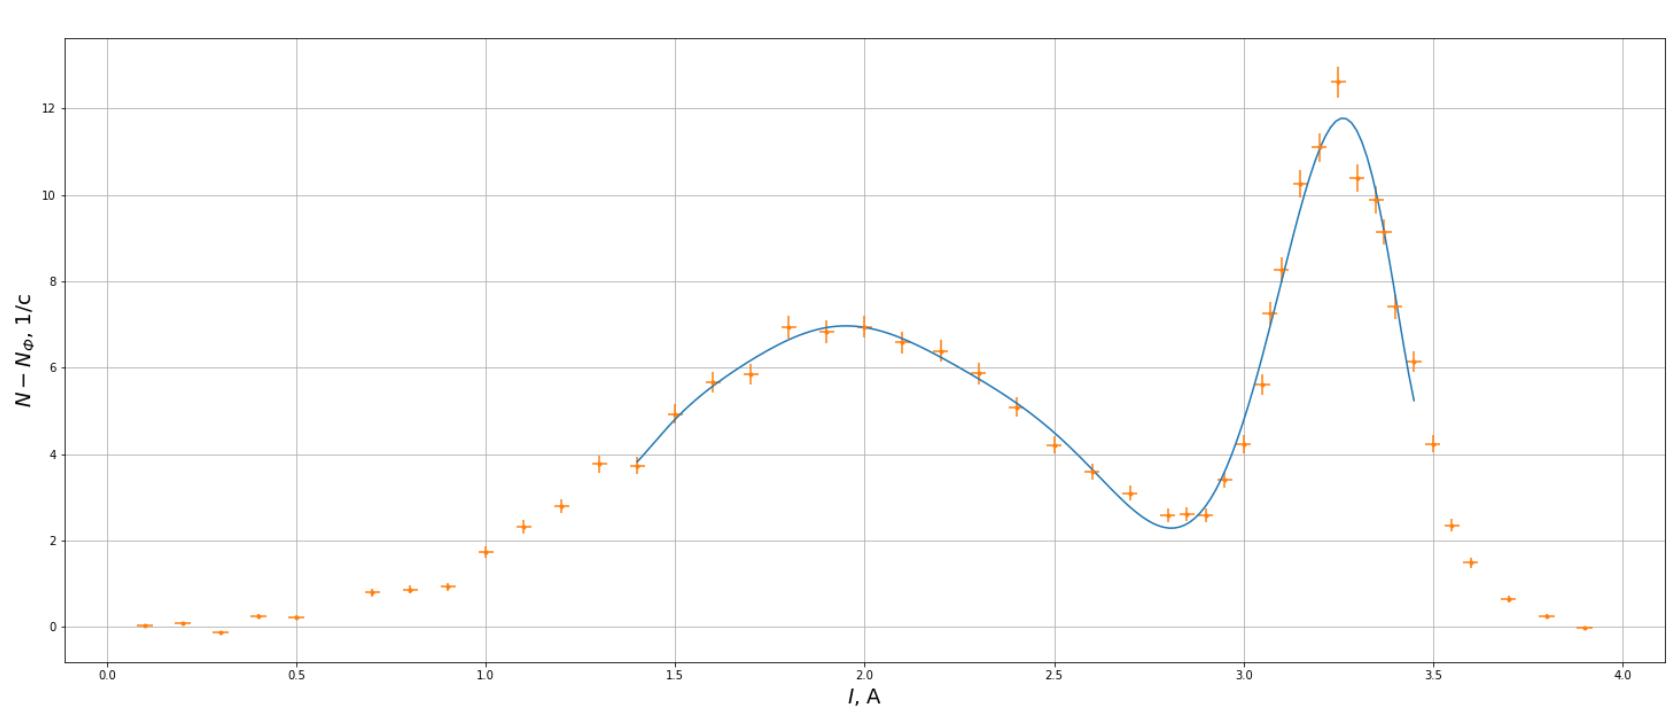
\includegraphics[width=\linewidth]{N_without_background.png}
  \caption{Измерение $\beta$-спектра.}
  \label{img::N_without_background}
\end{figure}

Зная конверсионный пик и соответствующие ему импульс $ p_c = 1013 $ кэВ/с и
энергию $ T = 634 $ кэВ, мы можем откалибровать шкалу токов в шкалу импульсов и
энергий.

Из формулы \eqref{eq::dNdE} получим

\begin{equation}\label{}
  N(p) \approx p^3 (E_e - E)^2 \Rightarrow \dfrac{\sqrt{N}}{p^{3/2}} \propto T_{max} - T
\end{equation}

Отложив по оси $ y $ величину $ \dfrac{\sqrt{N}}{p^{3/2}} = f $, а по $ x $ ---
кинетическую энергию, мы можем построить график, называемый графиком Ферми-Кюри,
и определить по нему $ T_{max} $ --- в этих осях спектр $\beta$-распада
описывается прямой, который мы можем профитировать $ y = ax +b $.

\begin{figure}[h]
  \centering
  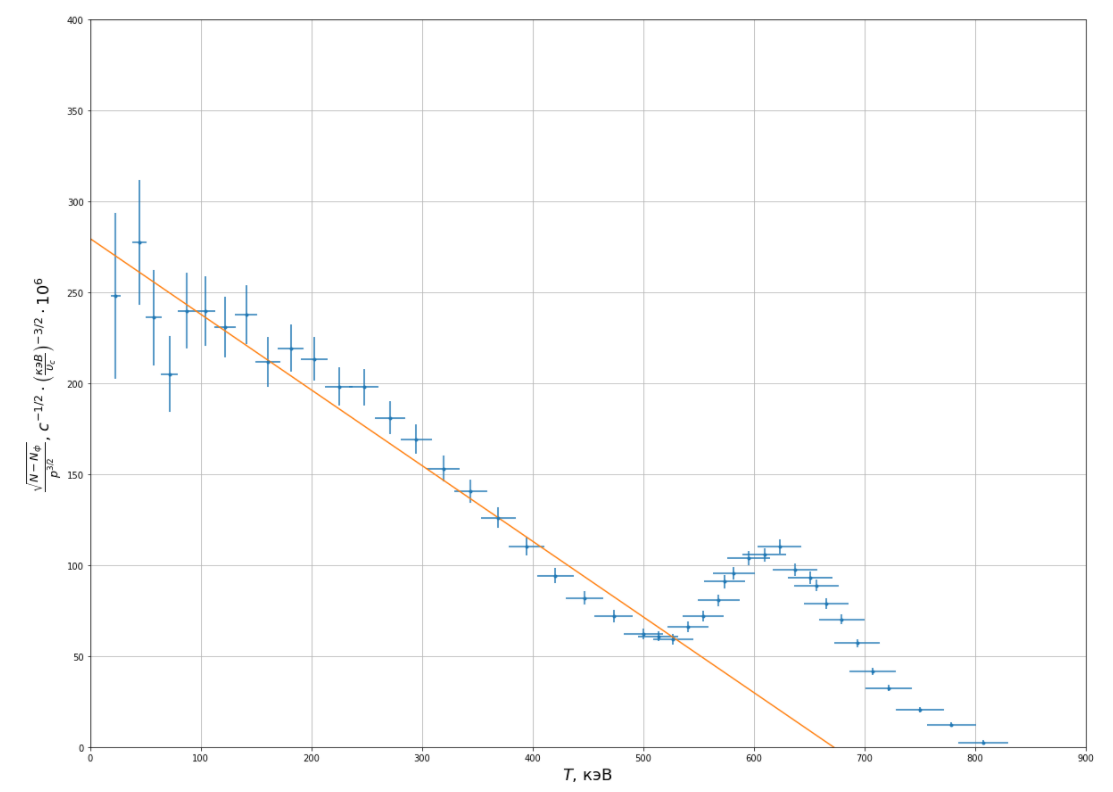
\includegraphics[width=\linewidth]{weirdo.png}
  \caption{График Ферми-Кюри}
  \label{img::N_without_background}
\end{figure}

В результате мы получаем, что $T_{max} = 672 \pm 64$ кэВ при $y = 0$.